\documentclass[runningheads]{llncs}
\usepackage{amsmath,amssymb}
\usepackage{graphicx}
\usepackage{todonotes,lineno}
\usepackage{paralist,soul}
\usepackage{rotating,multicol}
\usepackage{booktabs,tabularx}
\graphicspath{{figures/}}
\usepackage[font=small,labelfont=small]{subcaption}
\usepackage[font=small,labelfont=bf,format=plain]{caption}
\usepackage[pdfpagelabels,colorlinks,citecolor=blue,linkcolor=blue,urlcolor=blue]{hyperref}

\newcommand{\tabularbefore}{\vspace{4pt}\noindent}
\newcommand{\tabularafter}{\vspace{4pt}}
\newcommand{\myparagraph}[1]{\medskip\noindent\textbf{#1}.}
\newcommand\rurl[1]{\href{http://#1}{\nolinkurl{#1}}}

% ==================================================================
\author{Michael~A.~Bekos, Mirco~Haug, Michael~Kaufmann, Julia~M\"annecke}

\authorrunning{M.~A.~Bekos, M.~Haug, M.~Kaufmann, J.~M\"annecke}
\title{An Online Framework to Interact and Efficiently Compute Linear Layouts of Graphs} 
\titlerunning{An Online Framework to Interact and Compute Efficiently Linear Layouts}

\institute{
Institut f\"ur Informatik, Universit\"at T\"ubingen, T\"ubingen, Germany\\
\texttt{\{bekos,mk\}@informatik.uni-tuebingen.de}\\
\texttt{\{mirco.haug,julia.maennecke\}@student.uni-tuebingen.de}
}

% ==================================================================
\begin{document}
\maketitle
%\linenumbers
% ==================================================================

\begin{abstract}
We present a prototype online system to automate the procedure of computing different types of linear layouts of graphs under different user-specific constraints. The system consists of two main components; the client and the server sides. The client side is built upon an easy-to-use editor, which supports basic interaction with graphs, enriched with several additional features to allow the user to define and further constraint the linear layout to be computed. 

The server side, which is available to multiple clients through a well-documented API, is responsible for the actual computation of the linear layout. Its algorithmic core is an extension of a SAT formulation~\cite{DBLP:conf/gd/Bekos0Z15}~that is known to be robust enough to solve non-trivial instances in reasonable amount of time. However, it  has also several known limitations and potential improvements that~we address in this work (e.g., limited applicability to a particular type of linear layouts, no support for additional constraints, limited extendability e.t.c.). 

As a proof of concept, we present our findings for a sketch of a proof of an important result in the field that was proposed by Yannakakis~\cite{DBLP:conf/stoc/Yannakakis86} back in 1986 (whose details, however, have not been published so far).
\end{abstract}

% ==================================================================
\section{Introduction}
\label{sec:introduction}
% ==================================================================

Linear layouts of graphs have been fruitful subjects of intense research over the years, both from a combinatorial and from an algorithmic point of view, as they play an important role in various fields; see, e.g.,~\cite{DBLP:journals/dmtcs/DujmovicW04}. Formally, a linear layout of graph $G=(V,E)$ consists of a linear order of its vertices (that is, a bijective function $\sigma: V \rightarrow \{1,\ldots,|V|\}$), and a partition of its edges into a particular number of sets. Different constraints on the edges that may reside in the same set, give rise to different types of linear layouts; see, e.g.,~\cite{DBLP:conf/wg/AlamBG0P18,DBLP:journals/ejc/BinucciGHL18,DBLP:journals/siamcomp/HeathR92,DBLP:conf/gd/Pupyrev17,DBLP:journals/jcss/Yannakakis89}. In particular, there is a rich body of research on two specific types of linear layouts; the stack and the queue layouts. 

In a \emph{stack} (\emph{queue}) \emph{layout} of a graph, no two edges of the same set, called \emph{stack} (\emph{queue}) in this context, are allowed to cross (nest, respectively)~\cite{DBLP:journals/siamcomp/HeathR92,DBLP:journals/jcss/Yannakakis89}, where two edges $(u,v)$ and $(w,z)$, such that $\sigma(u)<\sigma(v)$ and $\sigma(w)<\sigma(z)$, \emph{cross} if $\sigma(u)<\sigma(w)<\sigma(v)<\sigma(z)$, and \emph{nest} if $\sigma(u)<\sigma(w)<\sigma(z)<\sigma(v)$; see, e.g., Fig.~\ref{fig:sample}. The \emph{stack-number} (\emph{queue-number}) of a graph is the minimum number of stacks (queues) required by any of its stack layouts (of its queue layouts, respectively). Note that stack layouts are widely known also as \emph{book embeddings}. 

\begin{figure}[t]
	\centering
	\subcaptionbox{\label{fig:goldner-harary}}{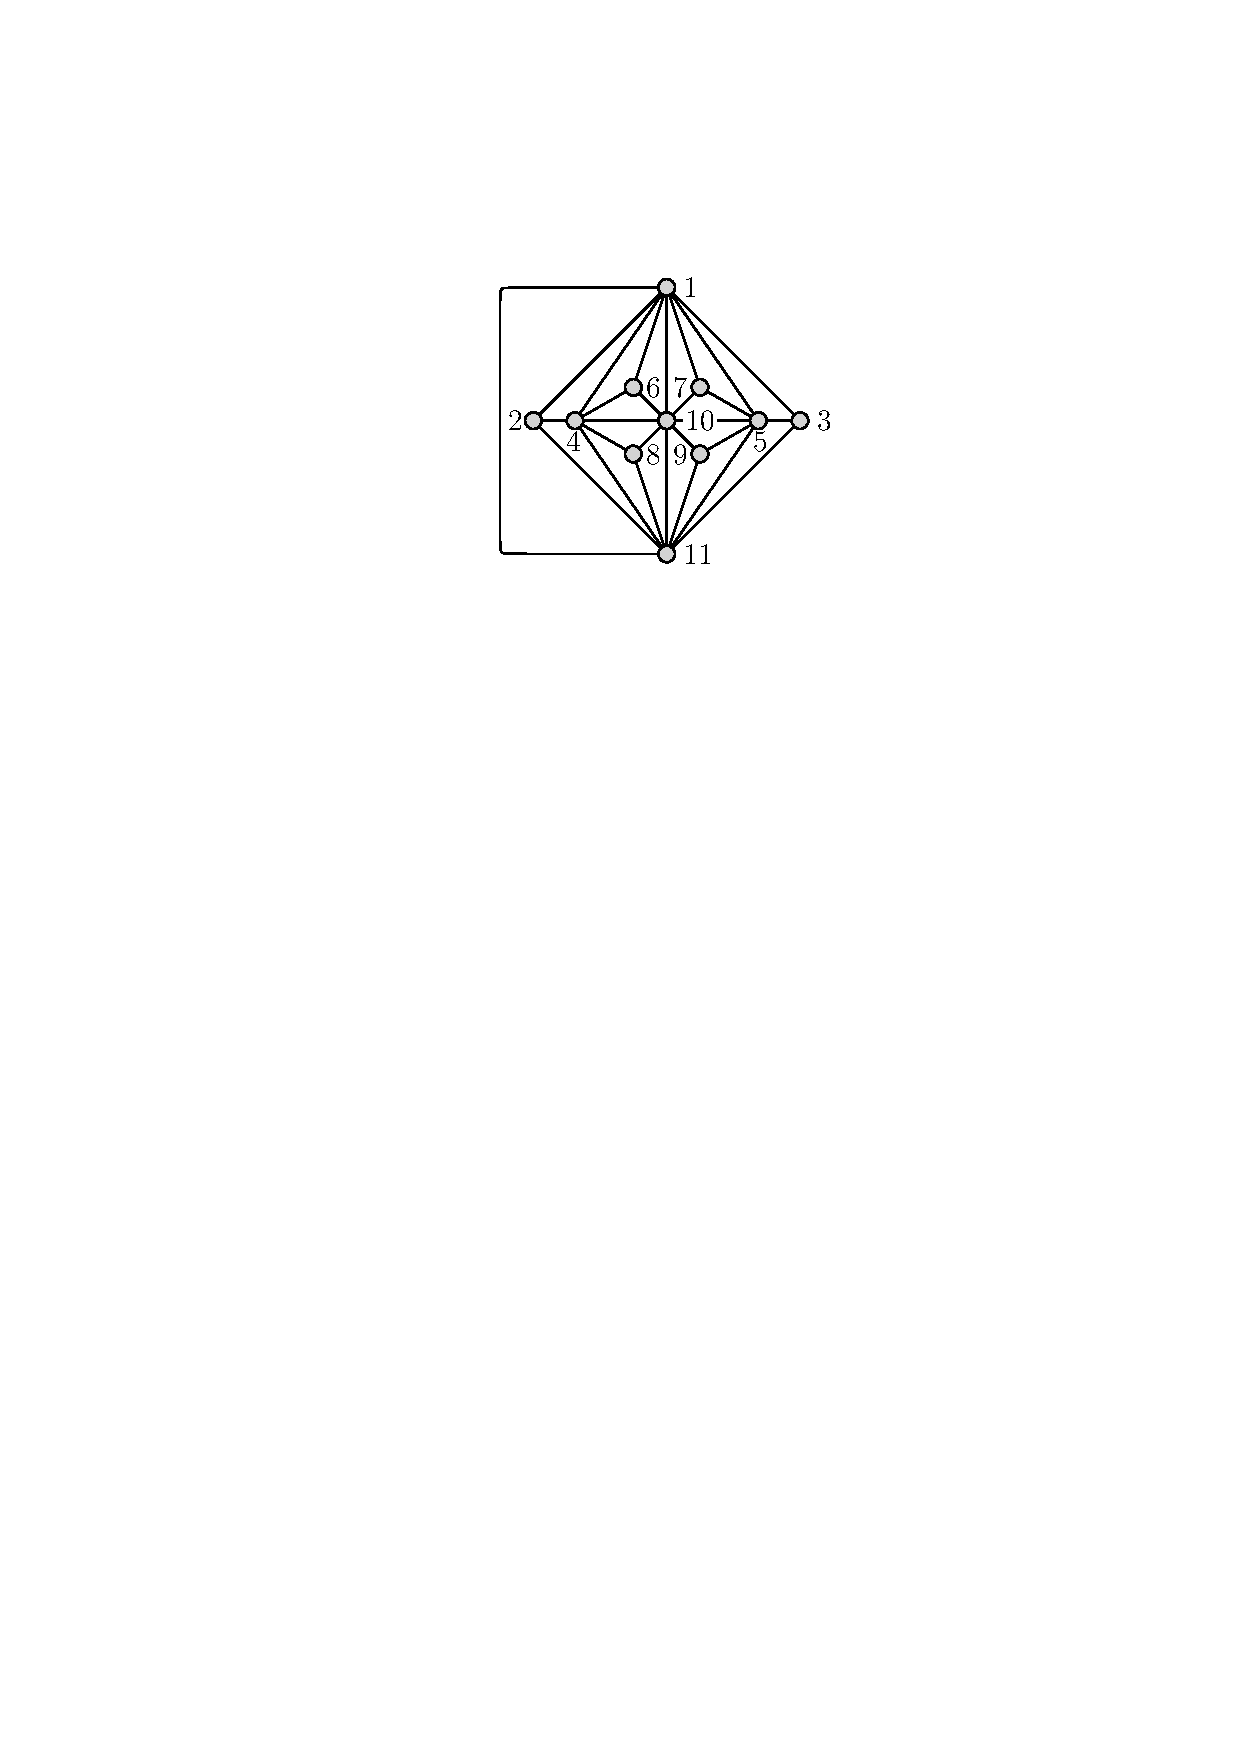
\includegraphics[width=0.172\textwidth,page=1]{graphs}}
	\hfil
	\subcaptionbox{\label{fig:stack}}{\includegraphics[width=0.4\textwidth,page=2]{graphs}}
	\hfil
	\subcaptionbox{\label{fig:queue}}{\includegraphics[width=0.4\textwidth,page=3]{graphs}}
   \caption{%
   Illustration of:   
   (a)~the Goldner-Harary graph~\cite{GH75},  
   (b)~a $3$-stack layout of it, and
   (c)~a $2$-queue layout of it.}
\label{fig:sample}
\end{figure}

\myparagraph{Known Results} There exists a plethora of theoretical results for each of the aforementioned types of linear layouts; in the following, we overview existing results for planar graphs, which is mainly the focus of our work. For a more detailed overview, we point the reader to~\cite{DBLP:journals/dmtcs/DujmovicW04}. 
%
\begin{itemize}[--]
\item For stack layouts, the most notable result is to due Yannakakis, who back in 1986 showed that every planar graph admits a $4$-stack layout~\cite{DBLP:conf/stoc/Yannakakis86,DBLP:journals/jcss/Yannakakis89} improving a series of earlier results~\cite{DBLP:conf/stoc/BussS84,DBLP:conf/focs/Heath84,Istrail1988a}. However, a fundamental question, which still remains open in the field, is whether every planar graph admits a $3$-stack layout or whether there exists one which requires four stacks in any of its stack layouts. Note that several subfamilies of planar graphs allow for layouts with fewer than four stacks; see, e.g.,~\cite{DBLP:journals/algorithmica/BekosGR16,DBLP:journals/jct/BernhartK79,DBLP:journals/mp/CornuejolsNP83,DBLP:journals/dcg/FraysseixMP95,Ewald1973,DBLP:conf/focs/Heath84,DBLP:journals/appml/KainenO07,NC08,DBLP:conf/cocoon/RengarajanM95}. 
\item For queue layouts, a breakthrough result is due to Dujmovi\'c et al.~\cite{constant}, who recently showed that every planar graph admits a $49$-queue layout, improving previous (poly-)logarithmic bounds~\cite{DBLP:journals/corr/BannisterDDEW18,DBLP:journals/jgaa/DujmovicF18,DBLP:journals/siamcomp/BattistaFP13}; the best-known corresponding lower bound is four~\cite{DBLP:conf/gd/AlamBG0P18}, which implies that the current gap between the two bounds is still very large. Again, several subfamilies of planar graphs allow for layouts with significantly fewer than $49$ queues; see, e.g.,~\cite{DBLP:conf/gd/AlamBG0P18,Ganley95,DBLP:journals/siamdm/HeathLR92,DBLP:journals/siamcomp/HeathR92,DBLP:conf/cocoon/RengarajanM95}.
\end{itemize}
%
\myparagraph{Motivation} The primary motivation of this project stems from the aforementioned paper by Yannakakis, which had appeared at STOC in 1986~\cite{DBLP:conf/stoc/Yannakakis86} and contained a sketch of a proof for the existence of a planar graph that does not admit a $3$-stack layout (we provide an outline of this sketch in Section~\ref{subsec:Yannakakis}). The details of this proof, however, never appeared in a paper (in particular, the proof-sketch was not part of the subsequent journal version~\cite{DBLP:journals/jcss/Yannakakis89} of the extended abstract that had appeared at STOC~\cite{DBLP:conf/stoc/Yannakakis86}), and thus the problem of determining whether there exists a planar graph that requires four stacks in any of its stack layouts still remains unsolved, and clearly forms the most intriguing open problem~in~the~field. Note that the arguments in the proof-sketch by Yannakakis~\cite{DBLP:conf/stoc/Yannakakis86} seem to be sound (apart from the fact that some of the gadget-graphs that are central in the proof have not been properly defined), and potentially may give rise to a formal proof. 

So, in this work we wanted to dig the details of this proof-sketch, so to understand if (and more importantly where) the proof fails. In addition, we were interested in finding the claimed gadget-graphs, which are not given in the proof. To this end, we decided to continue working on a SAT formulation~\cite{DBLP:conf/gd/Bekos0Z15}, that we proposed few years ago (for the problem of finding a stack layout of a given graph with a certain number of stacks), which we had to extend with several new features that are of independent value, even for future considerations.

\myparagraph{Contribution} The main contribution of this work is a novel system, which is available online (\rurl{algo.inf.uni-tuebingen.de/linearlayouts}) and automates the procedure of computing different types of linear layouts of graphs (i.e., stack layouts, queue layouts or mixtures of these). Besides the description of the system and its functions, we deem important to stress how the extensions that we propose stem from realistic problems that we encountered, while trying to check the different parts of the proof-sketch by Yannakakis~\cite{DBLP:conf/stoc/Yannakakis86}. The first major issue that we encountered was the need to define additional constraints  on the layouts to be computed (e.g., on the relative order of the vertices, or on the edges to appear at specific pages e.t.c.), that is, without, e.g., writing lines of code tailored to each of these constraints. A second major issue was the need to interact with the graph, that we were investigating, as efficiently as possible. To this end, we featured the system with an easy-to-use graph editor, which supports basic interaction with graphs, and simultaneously provides the necessary functionality to define and further constraint the linear layouts to be computed. Overall, we believe that the real value of the system is that, at its current state, it automates several of the standard procedures that a domain expert needs when interacting with linear layouts~of~graphs.

\myparagraph{Paper Organization} In Section~\ref{sec:system}, we describe in details the extended features that we have implemented in the system together with some insights on the SAT formulation. Section~\ref{sec:proof-of-concept} serves as a proof of concept for our system; we first present an outline of the  proof-sketch by Yannakakis mentioned above, and then we present our findings for the different parts of the proof-sketch. We conclude in Section~\ref{sec:conclusions} with further considerations and plans.

 
% ==================================================================
\section{Description of the System}
\label{sec:system}
% ==================================================================

Our system, as introduced in Section~\ref{sec:introduction}, consists of two main components, the client and the server sides, and introduces a series of innovations over its previous implementation~\cite{bob}. The actual code of the system is available to the community at a \texttt{github} repository (\rurl{github.com/linear-layouts/SAT}). In the following, we describe in details the extended features that are currently supported both in the client (Section~\ref{subsec:client}) and the server side (Section~\ref{subsec:server}). 

% ==================================================================
\subsection{The Client Side}
\label{subsec:client}
% ==================================================================

\begin{figure}[t]
	\centering
	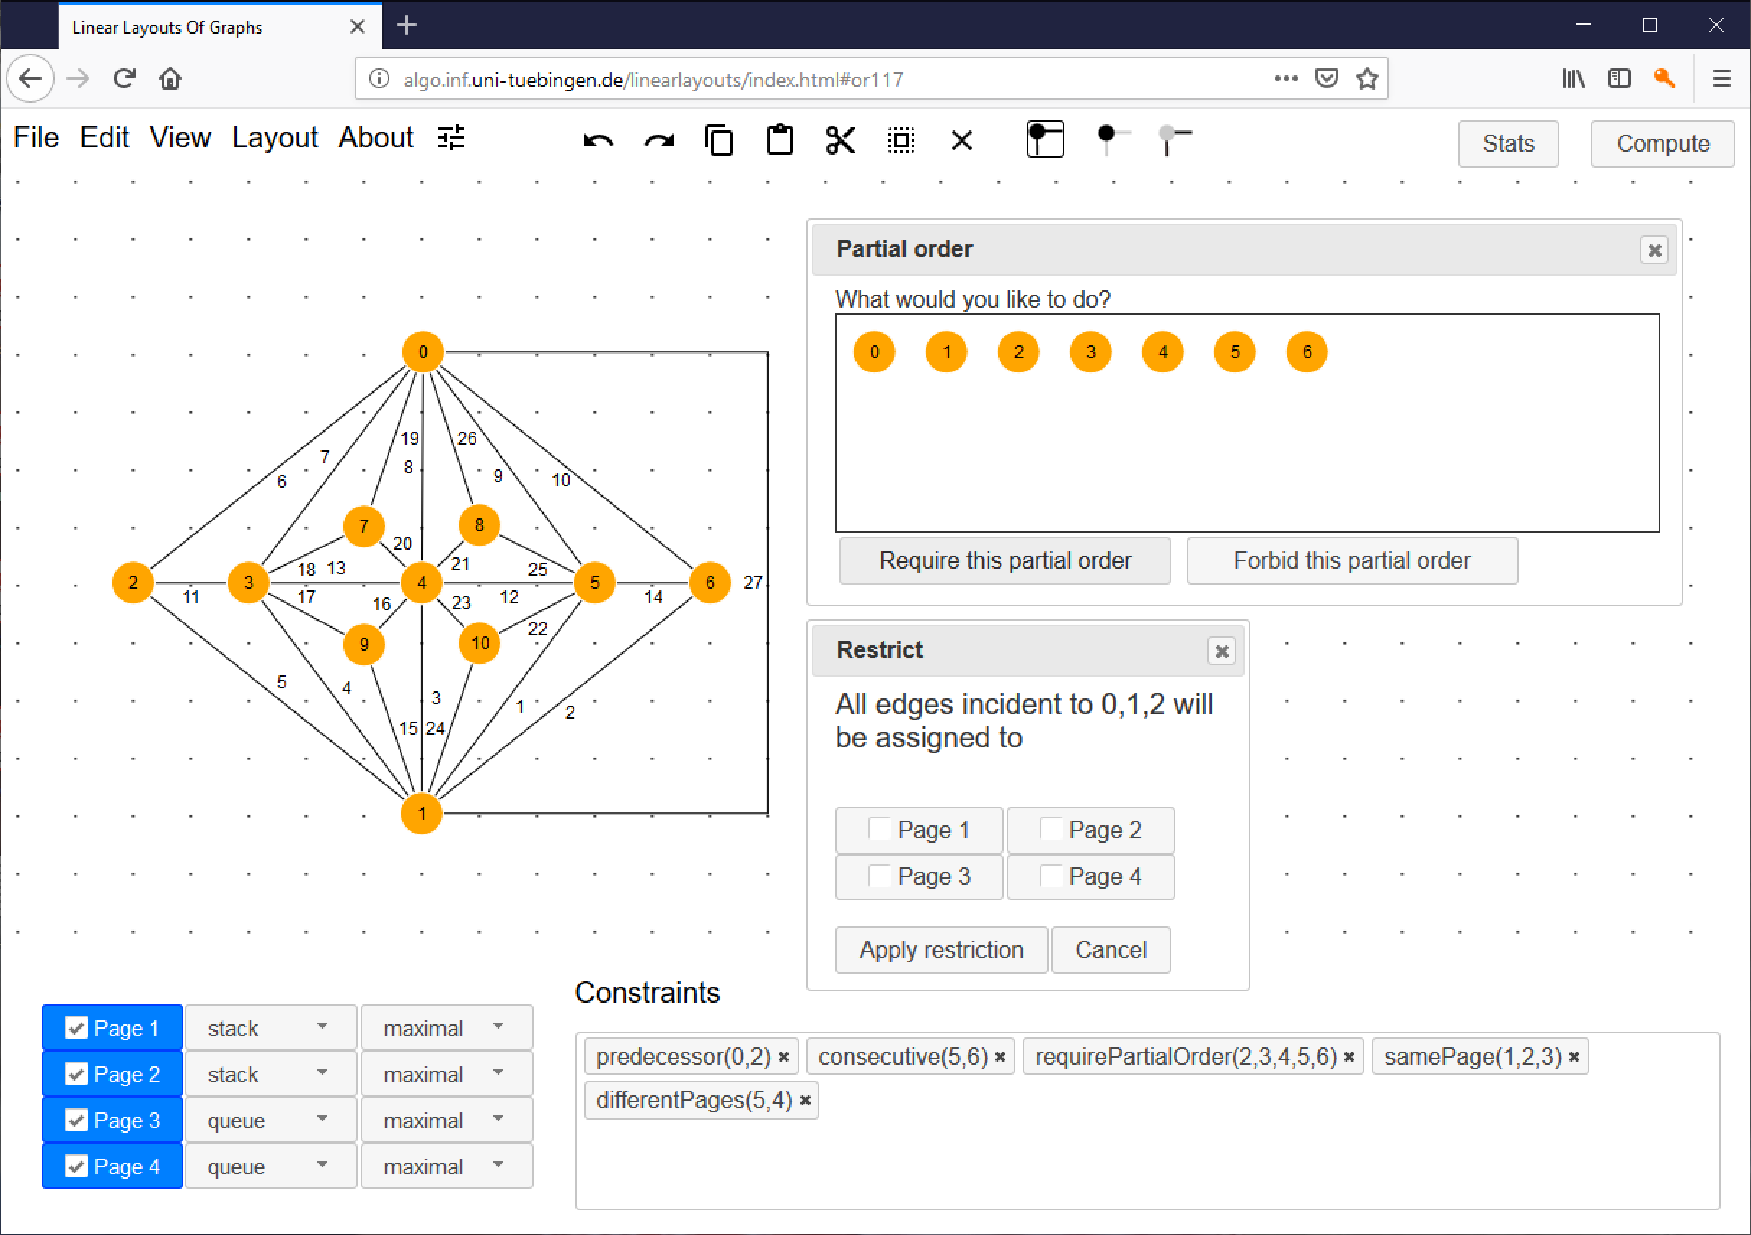
\includegraphics[width=\textwidth]{editingmode}
	\caption{A screenshot of the system in editing mode.}
	\label{fig:editingmode}
\end{figure}

The client side is web-based, developed with standard tools (e.g., \texttt{HTML}, \texttt{jQuery} and \texttt{yFiles}~\cite{DBLP:conf/gd/WieseEK00}, which is free for academic usage) and operates in two modes; the \emph{editing} and the \emph{view} (see Figs.~\ref{fig:editingmode} and~\ref{fig:viewmode}).  In the editing mode, the user creates the graph and specifies the constraints of the linear layout to be computed (if any). The graph is created through a graph editor supporting basic interaction with graphs (e.g., creation and deletion of vertices and edges, navigation over the graph, panning, zooming, e.t.c.), that we configured appropriately to meet our needs. The graph editor is accompanied with a \emph{configuration panel} (refer to the bottom part of Fig.~\ref{fig:editingmode}), where the user can configure the type of the layout, as well as, define different constraints on it. More precisely, the following functions are currently supported:

\myparagraph{Specification of the type of the linear layout} Through the configuration panel, the user defines the number of available \emph{pages} (i.e., stacks or queues) of the linear layout to be computed. The current implementation supports up to four pages, in total. In a subsequent step, the user defines the \emph{type} (i.e., stack or queue) of each of the pages of the linear layout. In this way, the system provides support both for stack and queue layouts, but also for \textit{mixed layouts}, in which some of the pages are stacks, while some others are queues; see, e.g,~\cite{DBLP:conf/gd/Pupyrev17}.

\myparagraph{Specification of structural constraints} In a stack (queue) layout of a graph, the subgraphs induced by the edges of each of its stacks (queues) are outerplanar~\cite{DBLP:journals/jct/BernhartK79} (arched-level planar~\cite{DBLP:journals/siamcomp/HeathR92}, respectively). 
%
Besides the number and the type of the available pages of the linear layout, the user can also impose additional structural constraints on these subgraphs. Currently, for each of the available pages, the user can choose one of the following options; not to impose any restriction on the subgraph induced by the edges of a particular page (apart from those that are necessarily imposed by the type of the page), or to restrict the subgraph induced by the edges of a particular page to be either a matching~or~a~tree.

\myparagraph{Imposition of restrictions on the linear order} There exist several ways to impose restrictions on the linear order of vertices of the linear layout (see Fig.~\ref{fig:options}). The constraints are created through the  editor and are stored in a separate component of the configuration panel (so that the user is able~to~remove~them). 

\begin{enumerate}[R.1]
\item \label{r:suc-pre} \textbf{Specification of successors and predecessors of vertices}: By selecting two vertices of the graph and by right-clicking on one of them, the user is able to set one of the selected vertices successor or predecessor of the other.
\item \label{r:consec} \textbf{Specification of vertices to be consecutive}: In the same way, the user is able to require two selected vertices to appear consecutively in the linear order of the vertices. Note that this constraint does not restrict the relative order of them. However, this can be easily achieved by combining Restrictions R.\ref{r:suc-pre} and~R.\ref{r:consec}. 
\item \label{r:order} \textbf{Specification of required and forbidden partial orders.}  By clicking on two or more vertices of the graph, while keeping the ctrl button of the keyboard pressed, the user is able to select multiple vertices in a specific order. Then, by right-clicking on one of them the system provides support to restrict the relative order of the selected vertices to be the one (or not to be the one), in which the vertices were clicked on. 
\end{enumerate}
%
\begin{figure}[t]
	\centering
	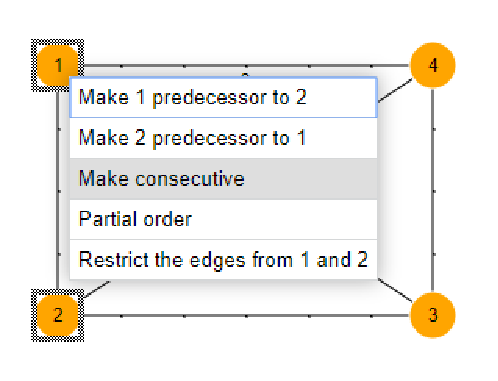
\includegraphics[width=0.3\textwidth,page=1]{options}
	\hfil
	\includegraphics[width=0.3\textwidth,page=2]{options}
   \caption{%
   A snapshot illustrating the options available on selected    
   vertices and edges.}
\label{fig:options}
\end{figure}
%
\noindent\textbf{Imposition of restrictions on the edge assignments.} Besides the restrictions on the linear order of the vertices, the user is also able to assign specific edges to particular pages. This can be achieved through the following functions.
%
\begin{enumerate}[R.1]
\setcounter{enumi}{3}
\item \label{r:edge-page} \textbf{Assignment of edges to the same or to different pages}: By selecting two or more edges of the graph and by right-clicking on one of them, the user is able to instruct the system to assign the selected edges to the same or to different pages of the linear layout. Note that the latter option becomes unavailable, when the number of selected edges is greater than the number of available pages of the linear layout. 
\item \label{r:same-page} \textbf{Assignment of edges to specific pages}: In the same way as above, the user is able to assign selected edges of the graph to one of a set of specific pages of the linear layout. In contrast to Restriction R.\ref{r:edge-page}, the user here has to specify the exact pages, to which the selected pages will be assigned. 
\item \label{r:incident} \textbf{Assignment of edges incident to vertices to specific pages}: The user is also able to assign edges to specific pages through a selection of vertices; in particular, the edges incident to these vertices. In the special case, in which the selected vertices are only two, say $u$ and $v$, then in the linear order of the vertices, $u$ and $v$ define two intervals; the one between $u$ and $v$, and the remaining one. In this particular case, the user is also able to apply the constrain only to the edges from $u$ and $v$ that end to only one of these two intervals. 
\end{enumerate}
%
\myparagraph{Additional features} The editing mode is equipped with several additional features; in the following, we name few. In order to facilitate the definition of the constraints on the different elements of the graph, the user may restrict the selection mode of the graph editor only to vertices or only to edges, depending on the type of constraints that she wish to introduce. The user is able to save both the graph and its associated constraints in a \texttt{GraphML} file for future considerations (see, e.g., \rurl{graphml.graphdrawing.org}). There exist also two options that are currently supported for exporting the constructed graph; one in \texttt{PDF} and one in \texttt{PNG} format. As side features, the editing mode is also equipped with standard layout algorithms (such as, spring-based, orthogonal and radial), while there is also support for querying the graph for standard properties (e.g., connectivity, acyclicity and planarity). 

\begin{figure}[t]
	\centering
	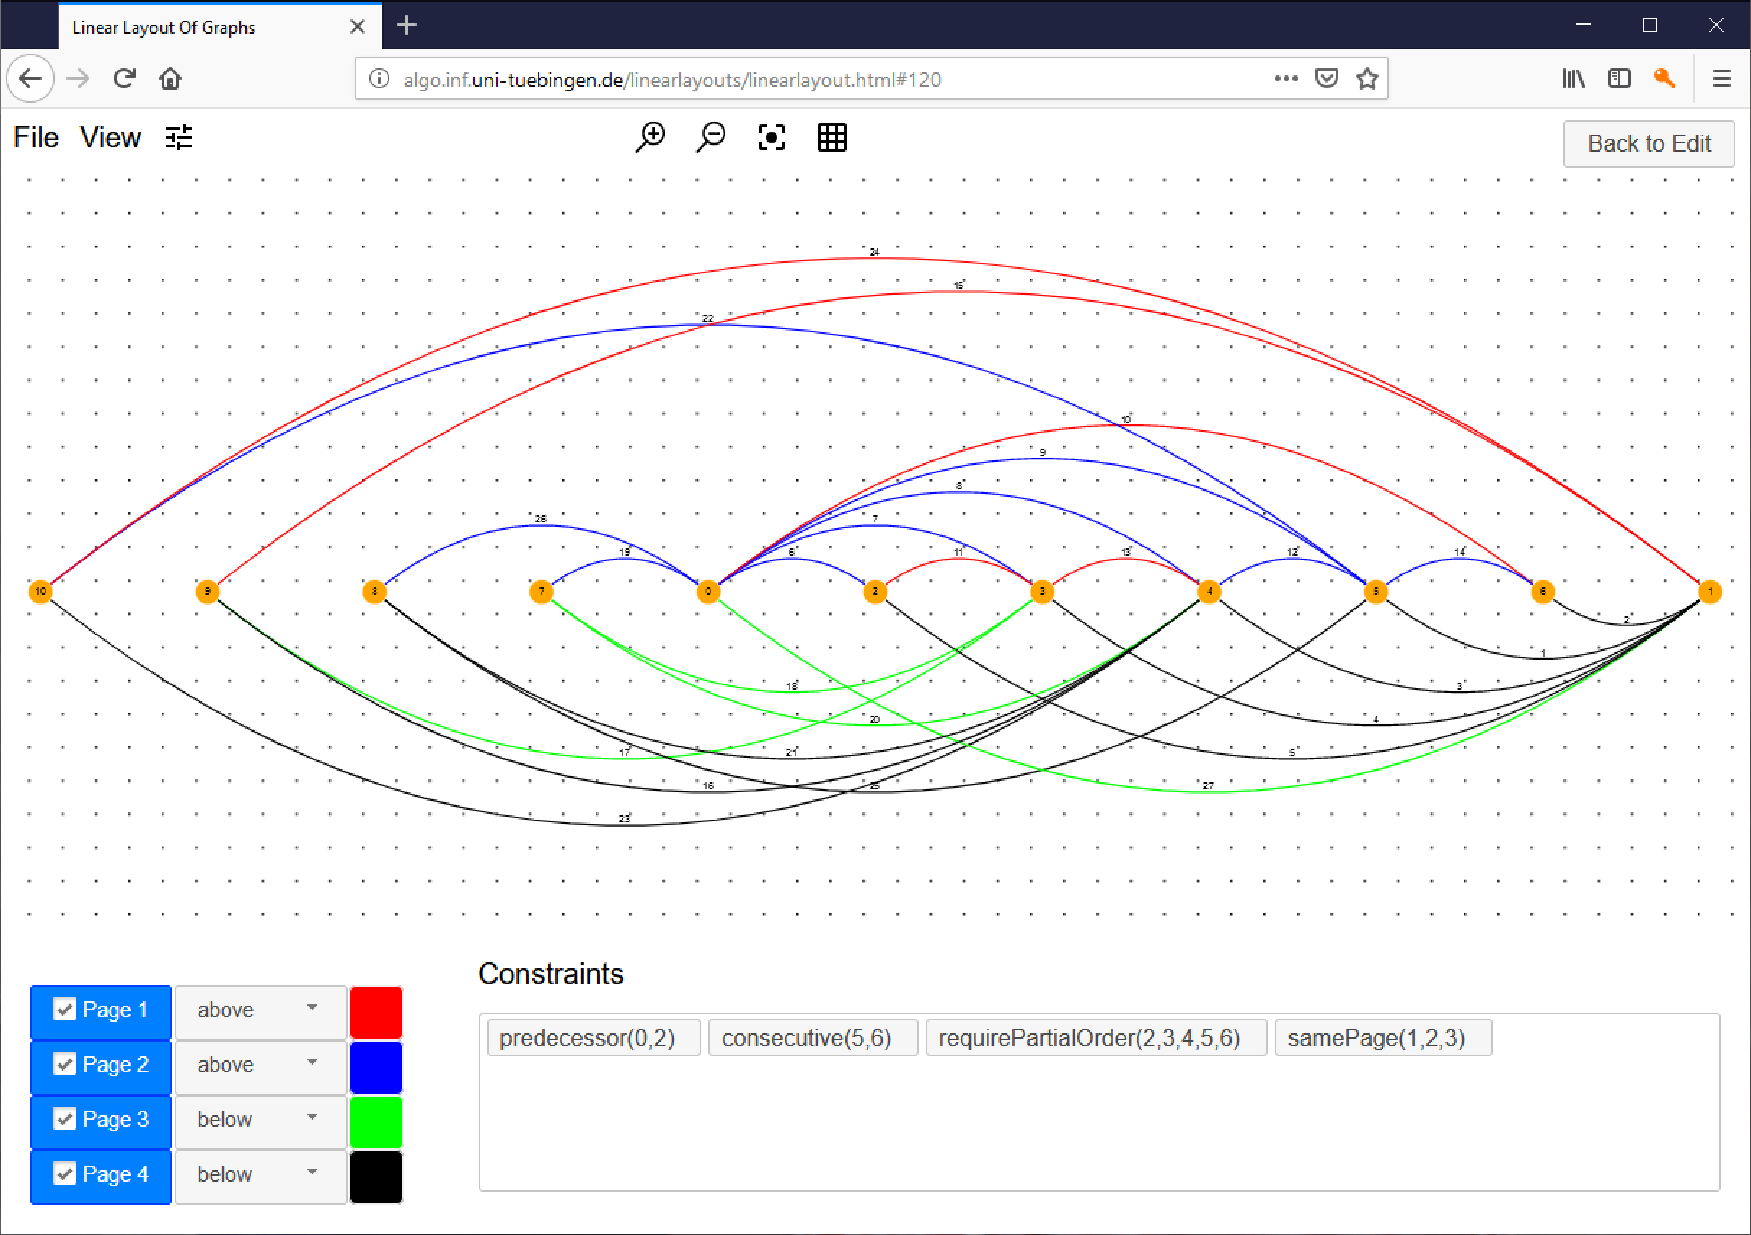
\includegraphics[width=\textwidth]{viewmode}
	\caption{A screenshot of the system in view mode.}
	\label{fig:viewmode}
\end{figure}

Once the creation of the graph and the definition of the constraints on its linear layout have been completed, the user may request to compute the actual linear layout (if any). At this point, the created graph and its constraints are passed to the server side, which is responsible for the actual computation. Once the computation has been completed, the system enters the view mode, where the computed linear layout is presented to the user. In contrast to the editing mode, in the view mode the user can partially interact with the computed linear layout, e.g., 
\begin{inparaenum}[(i)]
\item change the common color and the placement (i.e., above or below the line, on which the vertices reside) of the edges assigned to each page,
\item save or export the final layout to a file, and 
\item navigate, pan or zoom over the layout.
\end{inparaenum}

If the user seeks in further editing the graph and its constraints, then she has to return back to the editing mode. In this transition, the user may choose to work either with the original layout that had constructed before or with the computed linear layout (the user's configurations are also restored). 

% ==================================================================
\subsection{The Server Side}\label{subsec:server}
% ==================================================================

The server side of the system has been developed in \texttt{Python}, while for solving the SAT instances, we used the \texttt{Lingeling} solver (\rurl{fmv.jku.at/lingeling}); the source code of the server side is also contained in the \texttt{github} repository mentioned earlier. All requests that arrive to the server are stored in a database (\texttt{SQLite}), which is responsible for associating each of them with a unique id. Once the processing of a request is finished, the computed layout is stored to the database, so to be available to the client at any time. Note that the server side becomes available to multiple clients through a well-documented API available at the server's interface (\rurl{alice.informatik.uni-tuebingen.de:5555}). In other words, any client, that complies with the developed interface, may communicate with the server side and request a linear layout of a given graph under a set of additional constraints that are currently supported at the server. 

The algorithmic core of the server side is an extension of the SAT formulation~\cite{DBLP:conf/gd/Bekos0Z15} mentioned in the introduction, featured with additional functions to overcome known limitations; in particular to support  different types of linear layouts and different types of user-specific constraints. Even though SAT formulations are of limited applicability, and therefore not so common, in graph drawing (with few notable exceptions; e.g.,~\cite{DBLP:conf/gd/BiedlBNNPR13,DBLP:conf/gd/ChimaniZ12,DBLP:conf/gd/GangeSM10}), in this particular scenario the formulation is robust enough to solve non-trivial instances in reasonable amount of time (and, as expected, its performance increases when additional constraints are imposed). In the remainder of this section, we give a short overview of the original formulation followed by a high-level description of the extensions~that~we~made. 

The original formulation makes use of three types of variables $\sigma$, $\phi$ and~$\chi$~with the following meanings: 
\begin{inparaenum}[(i)]
\item for a pair of vertices $u$ and $v$, variable $\sigma(u,v)$ is $\texttt{true}$ if and only if $u$ precedes $v$ in the linear order, 
\item for an edge $e$ and a page $\rho$, variable $\phi_\rho(e)$ is $\texttt{true}$ if and only if edge $e$ is assigned to page $\rho$ of the layout, and 
\item for a pair of edges $e$ and $e'$, variable $\chi(e,e')$ is $\texttt{true}$ if and only if $e$ and $e'$ are assigned to the same page.
\end{inparaenum}  
So, there exist $O(n^2+m^2+pm)$ variables, where $n$ denotes the number of vertices of the graph, $m$ its number of edges, and $p$ the number of available pages. A set of $O(n^3+m^2)$ clauses ensure that the underlying order is linear, and that the layout is valid; for  details, refer to~\cite{DBLP:conf/gd/Bekos0Z15}.

To support different types of layouts, each page $\rho$ is associated with a \emph{type} $\tau(\rho)\in\{\text{\texttt{stack}, \texttt{queue}}\}$. If $\tau(\rho)=\text{\texttt{stack}}$, then we employ the same set of constraints as in the original formulation to avoid crossings in page $\rho$. Otherwise, $\tau(\rho)=\text{\texttt{queue}}$ holds, in which case we need to guarantee that no two edges of page $\rho$ nest. This can be ensured by introducing the following constraint for every pair of edges $(u,v)$ and $(z, w)$, such that $u$, $v$, $z$ and $w$ are pairwise different.

\tabularbefore
\begin{tabular}{ll}
$\phi_\rho(u,v) \wedge \phi_\rho(z,w))$ $\rightarrow$ &  
  $\neg (\sigma(u,z) \wedge \sigma(z,w) \wedge \sigma(w,v))~\wedge$\\
& $\neg (\sigma(u,w) \wedge \sigma(w,z) \wedge \sigma(z,v))~\wedge$\\
& $\neg (\sigma(v,z) \wedge \sigma(z,w) \wedge \sigma(w,u))~\wedge$\\ 
& $\neg (\sigma(v,w) \wedge \sigma(w,z) \wedge \sigma(z,u))$\\
\end{tabular}
\tabularafter

\noindent To ensure Restrictions~R.\ref{r:suc-pre}--R.\ref{r:order}, we introduce further constraints. Recall that R.\ref{r:suc-pre} and~R.\ref{r:consec} apply on a pair of vertices, denoted by $u$ and $v$ in the following, while R.\ref{r:order} applies on an ordered set of vertices, denoted by $\{u_1,\ldots,u_k\}$.

\tabularbefore
\begin{tabular}{@{}lrl}
R.\ref*{r:suc-pre}:~ & $\sigma(u,v)$, & ~if $u$ must be the predecessor of $v$ \\
& $\sigma(v,u)$, & ~otherwise \\
\end{tabular}
\tabularafter

\noindent
\begin{tabular}{@{}lrl}
R.\ref*{r:consec}:~ & $\sigma(x,u) \lor \sigma(v,x)$, & ~$\forall x \notin\{u,v\}$ \\
\end{tabular}
\tabularafter 

\noindent
\begin{tabular}{@{}lrl}
R.\ref*{r:order}: & $(\sigma(u_1,u_2)\wedge\ldots\wedge\sigma(u_{k-1},u_k))$, & if the order must be preserved\\ 
& $\neg(\sigma(u_1,u_2)\wedge\ldots\wedge\sigma(u_{k-1},u_k))$, & if the order must be avoided\\
\end{tabular}
\tabularafter

\noindent Restrictions~R.\ref{r:edge-page}--R.\ref{r:incident} are ensured in a similar fashion. Recall that R.\ref{r:edge-page} and~R.\ref{r:same-page} apply on an set of edges, denoted by $\{e_1,\ldots,e_\ell\}$ in the following, while R.\ref{r:incident} on an set of vertices, denoted by $\{u_1,\ldots,u_k\}$.

\tabularbefore
\begin{tabular}{@{}lrl}
R.\ref*{r:edge-page}:~ & $\chi(e,e'),\forall e,e'\in\{e_1,\ldots,e_\ell\}$, & ~if the edges must be in the same page\\
& $\neg\chi(e,e'),\forall e,e'\in\{e_1,\ldots,e_\ell\}$, & ~if the edges must be in different pages \\
\end{tabular}
\tabularafter

\noindent
\begin{tabular}{@{}lrl}
R.\ref*{r:same-page}:~ & $\neg\phi_{\rho}(e),\forall e \in \{e_1,\ldots,e_\ell\}$, & ~~~~~~~for each page $\rho$ that is not selected\\
\end{tabular}
\tabularafter

\noindent
\begin{tabular}{@{}lrl}
%R.\ref*{r:incident}:~ & $\neg\phi_{\rho}(e),\forall e \in \{(u,v): u\in\{u_1,\ldots,u_k\}\}$, & ~for each page $\rho$ that is not selected\\
R.\ref*{r:incident}:~ & $\neg\phi_{\rho}((u,\cdot)),\forall u \in \{u_1,\ldots,u_k\}$, & ~for each page $\rho$ that is not selected\\
\end{tabular}
\tabularafter

% ==================================================================
\section{Proof of Concept}
\label{sec:proof-of-concept}
% ==================================================================

In this section, we demonstrate how the system can be used by applying it to the proof-sketch by Yannakakis~\cite{DBLP:conf/stoc/Yannakakis86} that we mentioned in the introduction of the paper. At first, we give a short overview of this proof-sketch (Section~\ref{subsec:Yannakakis}), and then we described how we exploited the different functions of the system that we presented in Section~\ref{sec:system} to get meaningful insights of this proof-sketch (Section~\ref{subsec:findings}). We note at this point that the planar graph that Yannakakis claimed not to admit a $3$-stack layout is a tremendously large graph, since it is constructed by composing several smaller graphs, each of which has a certain property. Hence, testing via SAT (or via another such approach) whether this final graph admits a $3$-stack layout becomes realistically an impossible task. 

% ==================================================================
\subsection{An Overview of the Proof-Sketch by Yannakakis}
\label{subsec:Yannakakis}
% ==================================================================

In this section, we give an overview of the aforementioned proof-sketch~\cite{DBLP:conf/stoc/Yannakakis86} by Yannakakis that appeared as an extended abstract of~\cite{DBLP:journals/jcss/Yannakakis89} at STOC back in 1986. We deem important to stress at this point that since several parts of the proof-sketch have been omitted in~\cite{DBLP:conf/stoc/Yannakakis86}, the description of the main ideas of it are subject to the best of our understanding of the line of the arguments. 

The proof-sketch consists of three steps, each of which assumes the existence of a particular planar graph with a specific property. The graph of the first step, which we call \emph{skeleton}, consists of two designated vertices A and B that are connected to all the vertices of a long path $x_1 \rightarrow x_2 \rightarrow \ldots \rightarrow x_n$, which we call \emph{skeleton path}; for an illustration, refer to Fig.~\ref{fig:step-1}. The property of this graph is essentially the following: if $n$ is chosen large enough (e.g., $n=1000$), then in any $3$-stack layout of the skeleton graph at least one pair of consecutive vertices of the skeleton path will appear between $A$ and $B$. The observation that gives rise to the second step of the proof-sketch is that if one triples the length of the skeleton path, then one may assume two pairs of consecutive vertices of the skeleton path to lie between $A$ and $B$, and so on. In other words, if $n$ is chosen large enough, then there exists a particular number of pairs of consecutive vertices of the skeleton path, say $\langle y_1, y_2\rangle \ldots \langle y_{2k-1},y_{2k} \rangle$, that lie between $A$ and $B$ in any $3$-stack layout of the skeleton graph. 

\begin{figure}[t]
	\centering
	\subcaptionbox{\label{fig:step-1}Step 1}	
	{\includegraphics[scale=0.86,page=4]{graphs}}
	\hfil
	\subcaptionbox{\label{fig:step-2}Step 2}	
	{\includegraphics[scale=0.86,page=5]{graphs}}
	\hfil
	\subcaptionbox{\label{fig:step-3}Step 3}	
	{\includegraphics[scale=0.86,page=6]{graphs}}
   \caption{%
   Illustrations for the different steps of proof: 
   (a)~the skeleton graph, 
   (b)~the stellated-skeleton, and
   (b)~the operation of attaching three copies of graph $Q$ 
   along the edges of the subgraph of the stellated-skeleton 
   induced by $A$, $y_{2i_0-1}$, $a_{i_0}$,~$b_{i_0}$,~$y_{2i_0}$~and~$B$.}
   \label{fig:yannakakis}
\end{figure}

With this observation in mind, in the second step of the proof-sketch, the skeleton graph gets further augmented by \emph{stellating} each of its $2n$ triangular faces, that is, by adding a vertex in its interior and by connecting it to the three vertices of its boundary (refer to the gray-colored vertices in Fig.~\ref{fig:step-1}). Now, focus on the subgraph of the resulting graph, which we call \emph{stellated-skeleton}, that is induced by $A$,~$B$, $y_1,\ldots,y_{2k}$ and the vertices $a_1,\ldots,a_k$ and $b_1,\ldots,b_k$ that stellate the faces $\langle A, y_1, y_2\rangle\ldots\langle A, y_{2k-1}, y_{2k}\rangle$ and $\langle B, y_1, y_2\rangle\ldots\langle B, y_{2k-1}, y_{2k}\rangle$, respectively; see Fig.~\ref{fig:step-2}. The property of the stellated-skeleton is essentially the following.  If ($n$ is chosen sufficiently large such that) $k$ is large enough, then there exists a $4$-tuple $\langle y_{2i_0-1}, a_{i_0}, b_{i_0}, y_{2i_0}\rangle$ of vertices that appear in this order between $A$ and $B$ in any $3$-stack layout of the graph constructed so far.

The third step of the proof-sketch yields another augmentation to the graph, which is based on an internally-triangulated planar graph, denoted by $Q$ in~\cite{DBLP:conf/stoc/Yannakakis86}, whose outer face is bounded by a $4$-cycle $(s,a,t,b)$. In particular, three copies of graph $Q$ are ``attached'' along each edge $(u,v)$ of the graph that has been  constructed so far, such that vertices $s$ and $t$ of each of the three copies are identified with the endvertices $u$ and $v$ of the edge $(u,v)$; see Fig.~\ref{fig:step-3} for an illustration of this operation along the edges of the subgraph of the stellated-skeleton induced by $A$, $y_{2i_0-1}$, $a_{i_0}$, $b_{i_0}$, $y_{2i_0}$ and $B$. 

Note that graph $Q$ is not specified in the proof-sketch; Yannakakis only describes the properties for this graph, which are as follows. Graph $Q$ does not admit a $3$-stack layout such that 
\begin{inparaenum}[(P.1)]
\item \label{p:1} $a$ and $b$ lie between $s$ and $t$ in the linear order of the vertices, and 
\item \label{p:2} none of the edges from $s$ and $t$ to the vertices that lie between $s$ and $t$ in the linear order of the vertices (i.e., including $a$ and $b$) can be assigned to the third stack of the layout.
\end{inparaenum}

The three steps described so far formed the difficult part in the proof-sketch; the remainder of it is relatively easier. More precisely, assuming that the $4$-tuple $\langle y_{2i_0-1}, a_{i_0}, b_{i_0}, y_{2i_0}\rangle$ of the second step of the proof-sketch is guaranteed, and that the graph $Q$ of the corresponding third step (with the claimed Properties~P.\ref{p:1} and~P.\ref{p:2}) exists, the rest of the proof is sound (and more importantly described in the sketch). Hence, putting all the pieces of this proof together reduces in determining whether the $4$-tuple $\langle y_{2i_0-1}, a_{i_0}, b_{i_0}, y_{2i_0}\rangle$ as well as the~graph~$Q$~exist.


% ==================================================================
\subsection{Our Findings}
\label{subsec:findings}
% ==================================================================

As already mentioned in the introduction, most of the extensions that we implemented in our system are motivated by our efforts to check the different parts (in particular, the three main steps) of the proof-sketch by Yannakakis. This will become clear in this section, where we report our findings and describe how the developed system helped us to obtain meaningful insights of this proof. 

\myparagraph{Our findings on the first step of the proof-sketch} The task here was rather clear; we had to check whether two consecutive vertices of the skeleton path will inevitably appear between the two designated vertices $A$ and $B$ of the skeleton graph in any of its $3$-stack layouts, when the length of the skeleton path is large enough. 
%
To check this, we created an instance of the skeleton graph with approximately $100$ vertices. Then, using restriction R.\ref{r:suc-pre}, we instructed our system to constrain the layout to be computed, such that: 
%
\begin{inparaenum}[(i)]
\item vertex A (vertex B) is a predecessor (successor, respectively) of every odd-indexed vertex of the skeleton path, and
\item vertex A (vertex B) is a successor (predecessor, respectively) of every even-indexed vertex of the skeleton path.
\end{inparaenum} 
%
If the system could not report a solution under these two constraints, then the claim would follow. However, this was not the case, as the system could easily report a solution, which was so symmetric that we were able to generalize it to all~skeleton~graphs;~see~Fig.~\ref{fig:c1}.

\begin{figure}[t]
   \centering
   \includegraphics[width=.80\textwidth,page=8]{graphs}
   \caption{%
   A $3$-stack layout of the skeleton graph in which no two consecutive vertices of the skeleton path lie between $A$ and $B$.}
   \label{fig:c1}
\end{figure}

\myparagraph{Our findings on the second step of the proof-sketch} Even though our findings on the first step of the proof-sketch were a bit discouraging, we found it necessary to continue digging the details of the proof-sketch. Our idea was that if our findings on the second step were more promising, then we could try to modify (e.g., somehow augment) the skeleton graph, and eventually manage to guarantee its property. So, we decided to proceed to check the second step of the proof-sketch, under the assumption that somehow we can guarantee the property of the first step, that is, several pairs of consecutive vertices $\langle y_1,y_2 \rangle, \ldots, \langle y_{2k-1}, y_{2k} \rangle$ of the skeleton path appear between the two designated vertices $A$ and $B$. 

Under this assumption, we had to check whether two stellating vertices $a_i$ and $b_i$ of two faces $\langle A, y_{2i-1}, y_{2i}\rangle$ and $\langle B, y_{2i-1}, y_{2i}\rangle$ of the stellated-skeleton will inevitably appear between $y_{2i-1}$ and $y_{2i}$, for some $i\in\{1,\ldots,k\}$. To check this, we created an instance of the stellated skeleton with approximately $100$ vertices (that is, $k \approx 25$). Then, employed restrictions R.\ref{r:suc-pre} and R.\ref{r:order} of our system to constrain the layout to be computed, such that: 
%
\begin{inparaenum}[(i)]
\item vertex A is a predecessor of all vertices of the graph,
\item vertex B is a successor of all vertices of the graph,
\item for every $i=1,\ldots,k$, the partial order $\langle y_{2i-1}, a_i, b_i, y_{2i} \rangle$ is forbidden, and
\item the same holds for the partial order $\langle y_{2i-1}, b_i, a_i, y_{2i} \rangle$.
\end{inparaenum} 
%
As it was the case with the first step of the proof-sketch, the system could report~a~solution, which was again symmetric and we were able to generalize it to all stellated skeletons; see Figure~\ref{fig:c2}.

\begin{figure}[t]
   \centering
   \includegraphics[width=.80\textwidth,page=9]{graphs}
   \caption{%
   A $3$-stack layout of the stellated-skeleton in which there exist no index $i\in\{1,\ldots,k\}$, such that the vertices $y_{2i-1}$, $a_{i}$, $b_{i}$, $y_{2i}$ appear in this order between~$A$~and~$B$.}
   \label{fig:c2}
\end{figure}
   
\myparagraph{Our findings on the third step of the proof-sketch} Finding a graph with the properties of the graph $Q$ in~\cite{DBLP:conf/stoc/Yannakakis86} was definitely a challenging task. In our efforts, we  crafted several internally-triangulated planar graphs with a quadrangular outer face, which contained substructures that are known to require a third stack, such as planar $3$-trees~\cite{DBLP:conf/focs/Heath84}, the Goldner-Harary graph~\cite{GH75} and planar graphs with several separating triangles~\cite{DBLP:journals/appml/KainenO07}. We also tested approximately 4.000 randomly generated planar graphs with 100 to 150 vertices, which we created by first triangulating an evenly distributed point set within a quadrangular region, and then by connecting four vertices at the corners of this region to all vertices on the (internally triangulated) point set without introducing crossings. Each of these graphs had by construction a quadrangular outer face $(s,a,t,b)$ and was tested for the property of graph $Q$ in~\cite{DBLP:conf/stoc/Yannakakis86} using restriction R.\ref{r:order} and R.\ref{r:incident} as follows: 
%
\begin{inparaenum}[(i)]
\item vertices $s$, $a$ and $t$ appear in this order, 
\item vertices $s$, $b$ and $t$ appear in this order, and
\item the edges from $s$ and $t$ that end in vertices between $s$ and $t$ are assigned to the first two pages of the layout.
\end{inparaenum} 

To put it briefly: we did not manage to find a graph with the claimed properties of graph $Q$ in~\cite{DBLP:conf/stoc/Yannakakis86}. As a matter of fact, in the layouts that we computed we observed that most of the times very few vertices were eventually between $s$ and $t$ (besides $a$ and $b$), which is an indication that the restrictions may not be strong enough. It is worth noting at this point that, in the original proof-sketch, it is mentioned that graph $Q$ is the endproduct of a series of constructions of smaller gadget-graphs $Q_1$, $Q_2$ and so forth (that are not described; actually, not even their properties are described), which is another indication that if a graph with the properties of graph $Q$ exists, then it might be tremendously large.
 

% ==================================================================
\section{Conclusions}
\label{sec:conclusions}
% ==================================================================

In this paper, we presented a novel system equipped with several features that automate most of the standard procedures that a domain expert needs for computing different types of (constrained) linear layouts of graphs. As a proof of concept, we used the developed system to check the different parts of a proof-sketch by Yannakakis~\cite{DBLP:conf/stoc/Yannakakis86}, and we managed to gain valuable insights. Our findings, of course, were mostly negative. The proposed system, however, might be useful in finding a suitable graph with the properties of graph $Q$ in~\cite{DBLP:conf/stoc/Yannakakis86} and some other graph (than the one Yannakakis proposed) yielding the $4$-tuple describe in Section~\ref{subsec:Yannakakis}. And so we are still hopeful that the proof-sketch can be completed. 

More in general, we believe that the developed system is extremely useful for proving lower bounds (e.g., to narrow the current wide gap between the upper and the lower bound on the queue number of planar graphs), which is the main reason to have it available online. We further plan to equip it with additional features, such as adding support for searching and filtering the layouts, highlighting the restrictions and more advanced definitions of restrictions.

\bibliographystyle{abbrvurl}
\bibliography{stacks,queues,bekos,general}

\end{document}
